\documentclass{standalone}
\usepackage{tikz}
\usepackage{ctex,siunitx}
\usepackage{tkz-euclide}
\usepackage{amsmath}
\usetikzlibrary{patterns, calc}
\usetikzlibrary {decorations.pathmorphing, decorations.pathreplacing, decorations.shapes,}
\begin{document}
\small
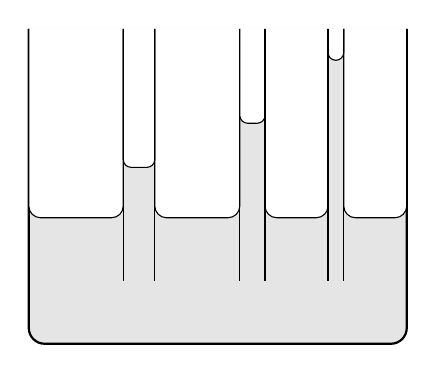
\begin{tikzpicture}[>=stealth,scale=0.8]
  \draw [fill=gray!20, rounded corners=0.2cm, thick](0,5)--(0, 0)--(6,0)--(6,5);
  \draw [fill=white, rounded corners=0.15cm](0,5)--(0,2)--(1.5,2)--(1.5,5);
  \draw [fill=white, rounded corners=0.15cm](2,5)--(2,2)--(3.35,2)--(3.35,5);
  \draw [fill=white, rounded corners=0.15cm](3.75,5)--(3.75,2)--(4.75,2)--(4.75,5);
  \draw [fill=white, rounded corners=0.15cm](5,5)--(5,2)--(6,2)--(6,5);
  \draw [fill=white, rounded corners=0.1cm](1.5, 5)--(1.5,2.8)--(2, 2.8)--(2,5);
  \draw [fill=white, rounded corners=0.1cm](3.35, 5)--(3.35,3.5)--(3.75, 3.5)-- (3.75, 5);
  \draw [fill=white, rounded corners=0.1cm](4.75, 5)--(4.75, 4.5)--(5, 4.5)--(5, 5);
  \foreach \x in {1.5,2,3.35,3.75,4.75,5}
  {
    \draw (\x, 1)--(\x, 5);
  }
\end{tikzpicture}
\end{document}